\section{CNo\-Such\-Object\-Exception  Class Reference}
\label{classCNoSuchObjectException}\index{CNoSuchObjectException@{CNo\-Such\-Object\-Exception}}
{\tt \#include $<$CNo\-Such\-Object\-Exception.h$>$}

Inheritance diagram for CNo\-Such\-Object\-Exception::\begin{figure}[H]
\begin{center}
\leavevmode
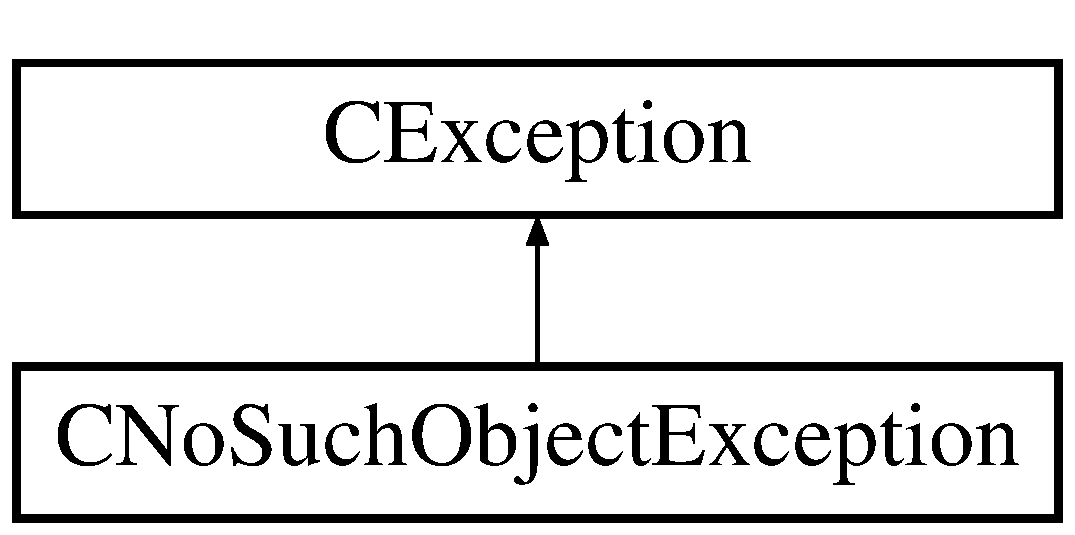
\includegraphics[height=2cm]{classCNoSuchObjectException}
\end{center}
\end{figure}
\subsection*{Public Methods}
\begin{CompactItemize}
\item 
{\bf CNo\-Such\-Object\-Exception} (const char $\ast$p\-Doing, const char $\ast$p\-Name)
\item 
{\bf CNo\-Such\-Object\-Exception} (const char $\ast$p\-Doing, const string \&r\-Name)
\item 
{\bf CNo\-Such\-Object\-Exception} (const string \&r\-Doing, const char $\ast$p\-Name)
\item 
{\bf CNo\-Such\-Object\-Exception} (const string \&r\-Doing, const string \&r\-Name)
\item 
virtual {\bf $\sim$CNo\-Such\-Object\-Exception} ()
\item 
{\bf CNo\-Such\-Object\-Exception} (const CNo\-Such\-Object\-Exception \&a\-CNo\-Such\-Object\-Exception)
\item 
CNo\-Such\-Object\-Exception {\bf operator=} (const CNo\-Such\-Object\-Exception \&a\-CNo\-Such\-Object\-Exception)
\item 
int {\bf operator==} (const CNo\-Such\-Object\-Exception \&a\-CNo\-Such\-Object\-Exception)
\item 
string {\bf get\-Name} () const
\item 
void {\bf set\-Name} (string am\_\-s\-Name)
\item 
virtual const char $\ast$ {\bf Reason\-Text} () const
\end{CompactItemize}
\subsection*{Protected Methods}
\begin{CompactItemize}
\item 
void {\bf Update\-Reason\-Text} ()
\end{CompactItemize}
\subsection*{Private Attributes}
\begin{CompactItemize}
\item 
string {\bf m\_\-s\-Name}
\item 
string {\bf m\_\-s\-Reason\-Text}
\end{CompactItemize}


\subsection{Constructor \& Destructor Documentation}
\index{CNoSuchObjectException@{CNo\-Such\-Object\-Exception}!CNoSuchObjectException@{CNoSuchObjectException}}
\index{CNoSuchObjectException@{CNoSuchObjectException}!CNoSuchObjectException@{CNo\-Such\-Object\-Exception}}
\subsubsection{\setlength{\rightskip}{0pt plus 5cm}CNo\-Such\-Object\-Exception::CNo\-Such\-Object\-Exception (const char $\ast$ {\em p\-Doing}, const char $\ast$ {\em p\-Name})\hspace{0.3cm}{\tt  [inline]}}\label{classCNoSuchObjectException_a0}




Definition at line 299 of file CNo\-Such\-Object\-Exception.h.

References m\_\-s\-Name, and Update\-Reason\-Text().\index{CNoSuchObjectException@{CNo\-Such\-Object\-Exception}!CNoSuchObjectException@{CNoSuchObjectException}}
\index{CNoSuchObjectException@{CNoSuchObjectException}!CNoSuchObjectException@{CNo\-Such\-Object\-Exception}}
\subsubsection{\setlength{\rightskip}{0pt plus 5cm}CNo\-Such\-Object\-Exception::CNo\-Such\-Object\-Exception (const char $\ast$ {\em p\-Doing}, const string \& {\em r\-Name})\hspace{0.3cm}{\tt  [inline]}}\label{classCNoSuchObjectException_a1}




Definition at line 304 of file CNo\-Such\-Object\-Exception.h.

References m\_\-s\-Name, and Update\-Reason\-Text().\index{CNoSuchObjectException@{CNo\-Such\-Object\-Exception}!CNoSuchObjectException@{CNoSuchObjectException}}
\index{CNoSuchObjectException@{CNoSuchObjectException}!CNoSuchObjectException@{CNo\-Such\-Object\-Exception}}
\subsubsection{\setlength{\rightskip}{0pt plus 5cm}CNo\-Such\-Object\-Exception::CNo\-Such\-Object\-Exception (const string \& {\em r\-Doing}, const char $\ast$ {\em p\-Name})\hspace{0.3cm}{\tt  [inline]}}\label{classCNoSuchObjectException_a2}




Definition at line 309 of file CNo\-Such\-Object\-Exception.h.

References m\_\-s\-Name, and Update\-Reason\-Text().\index{CNoSuchObjectException@{CNo\-Such\-Object\-Exception}!CNoSuchObjectException@{CNoSuchObjectException}}
\index{CNoSuchObjectException@{CNoSuchObjectException}!CNoSuchObjectException@{CNo\-Such\-Object\-Exception}}
\subsubsection{\setlength{\rightskip}{0pt plus 5cm}CNo\-Such\-Object\-Exception::CNo\-Such\-Object\-Exception (const string \& {\em r\-Doing}, const string \& {\em r\-Name})\hspace{0.3cm}{\tt  [inline]}}\label{classCNoSuchObjectException_a3}




Definition at line 314 of file CNo\-Such\-Object\-Exception.h.

References m\_\-s\-Name, and Update\-Reason\-Text().\index{CNoSuchObjectException@{CNo\-Such\-Object\-Exception}!~CNoSuchObjectException@{$\sim$CNoSuchObjectException}}
\index{~CNoSuchObjectException@{$\sim$CNoSuchObjectException}!CNoSuchObjectException@{CNo\-Such\-Object\-Exception}}
\subsubsection{\setlength{\rightskip}{0pt plus 5cm}virtual CNo\-Such\-Object\-Exception::$\sim$CNo\-Such\-Object\-Exception ()\hspace{0.3cm}{\tt  [inline, virtual]}}\label{classCNoSuchObjectException_a4}




Definition at line 319 of file CNo\-Such\-Object\-Exception.h.\index{CNoSuchObjectException@{CNo\-Such\-Object\-Exception}!CNoSuchObjectException@{CNoSuchObjectException}}
\index{CNoSuchObjectException@{CNoSuchObjectException}!CNoSuchObjectException@{CNo\-Such\-Object\-Exception}}
\subsubsection{\setlength{\rightskip}{0pt plus 5cm}CNo\-Such\-Object\-Exception::CNo\-Such\-Object\-Exception (const CNo\-Such\-Object\-Exception \& {\em a\-CNo\-Such\-Object\-Exception})\hspace{0.3cm}{\tt  [inline]}}\label{classCNoSuchObjectException_a5}




Definition at line 323 of file CNo\-Such\-Object\-Exception.h.

References m\_\-s\-Name, and Update\-Reason\-Text().

\subsection{Member Function Documentation}
\index{CNoSuchObjectException@{CNo\-Such\-Object\-Exception}!getName@{getName}}
\index{getName@{getName}!CNoSuchObjectException@{CNo\-Such\-Object\-Exception}}
\subsubsection{\setlength{\rightskip}{0pt plus 5cm}string CNo\-Such\-Object\-Exception::get\-Name () const\hspace{0.3cm}{\tt  [inline]}}\label{classCNoSuchObjectException_a8}




Definition at line 353 of file CNo\-Such\-Object\-Exception.h.

References m\_\-s\-Name.\index{CNoSuchObjectException@{CNo\-Such\-Object\-Exception}!operator=@{operator=}}
\index{operator=@{operator=}!CNoSuchObjectException@{CNo\-Such\-Object\-Exception}}
\subsubsection{\setlength{\rightskip}{0pt plus 5cm}CNo\-Such\-Object\-Exception CNo\-Such\-Object\-Exception::operator= (const CNo\-Such\-Object\-Exception \& {\em a\-CNo\-Such\-Object\-Exception})\hspace{0.3cm}{\tt  [inline]}}\label{classCNoSuchObjectException_a6}




Definition at line 333 of file CNo\-Such\-Object\-Exception.h.

References m\_\-s\-Name, CException::operator=(), and Update\-Reason\-Text().\index{CNoSuchObjectException@{CNo\-Such\-Object\-Exception}!operator==@{operator==}}
\index{operator==@{operator==}!CNoSuchObjectException@{CNo\-Such\-Object\-Exception}}
\subsubsection{\setlength{\rightskip}{0pt plus 5cm}int CNo\-Such\-Object\-Exception::operator== (const CNo\-Such\-Object\-Exception \& {\em a\-CNo\-Such\-Object\-Exception})\hspace{0.3cm}{\tt  [inline]}}\label{classCNoSuchObjectException_a7}




Definition at line 344 of file CNo\-Such\-Object\-Exception.h.

References m\_\-s\-Name, and CException::operator==().\index{CNoSuchObjectException@{CNo\-Such\-Object\-Exception}!ReasonText@{ReasonText}}
\index{ReasonText@{ReasonText}!CNoSuchObjectException@{CNo\-Such\-Object\-Exception}}
\subsubsection{\setlength{\rightskip}{0pt plus 5cm}const char $\ast$ CNo\-Such\-Object\-Exception::Reason\-Text () const\hspace{0.3cm}{\tt  [virtual]}}\label{classCNoSuchObjectException_a10}


Returns a const pointer to text which describes the reason the exception was thrown. This is exception type specific. The default action returns a pointer to the constant string: \char`\"{}Unspecified Exception\char`\"{} 

Reimplemented from {\bf CException} {\rm (p.\,\pageref{classCException_a8})}.

Definition at line 284 of file CNo\-Such\-Object\-Exception.cpp.

References m\_\-s\-Reason\-Text.\index{CNoSuchObjectException@{CNo\-Such\-Object\-Exception}!setName@{setName}}
\index{setName@{setName}!CNoSuchObjectException@{CNo\-Such\-Object\-Exception}}
\subsubsection{\setlength{\rightskip}{0pt plus 5cm}void CNo\-Such\-Object\-Exception::set\-Name (string {\em am\_\-s\-Name})\hspace{0.3cm}{\tt  [inline]}}\label{classCNoSuchObjectException_a9}




Definition at line 359 of file CNo\-Such\-Object\-Exception.h.

References m\_\-s\-Name.\index{CNoSuchObjectException@{CNo\-Such\-Object\-Exception}!UpdateReasonText@{UpdateReasonText}}
\index{UpdateReasonText@{UpdateReasonText}!CNoSuchObjectException@{CNo\-Such\-Object\-Exception}}
\subsubsection{\setlength{\rightskip}{0pt plus 5cm}void CNo\-Such\-Object\-Exception::Update\-Reason\-Text ()\hspace{0.3cm}{\tt  [protected]}}\label{classCNoSuchObjectException_b0}




Definition at line 290 of file CNo\-Such\-Object\-Exception.cpp.

References m\_\-s\-Name, and m\_\-s\-Reason\-Text.

Referenced by CNo\-Such\-Object\-Exception(), and operator=().

\subsection{Member Data Documentation}
\index{CNoSuchObjectException@{CNo\-Such\-Object\-Exception}!m_sName@{m\_\-sName}}
\index{m_sName@{m\_\-sName}!CNoSuchObjectException@{CNo\-Such\-Object\-Exception}}
\subsubsection{\setlength{\rightskip}{0pt plus 5cm}string CNo\-Such\-Object\-Exception::m\_\-s\-Name\hspace{0.3cm}{\tt  [private]}}\label{classCNoSuchObjectException_o0}




Definition at line 295 of file CNo\-Such\-Object\-Exception.h.

Referenced by CNo\-Such\-Object\-Exception(), get\-Name(), operator=(), operator==(), set\-Name(), and Update\-Reason\-Text().\index{CNoSuchObjectException@{CNo\-Such\-Object\-Exception}!m_sReasonText@{m\_\-sReasonText}}
\index{m_sReasonText@{m\_\-sReasonText}!CNoSuchObjectException@{CNo\-Such\-Object\-Exception}}
\subsubsection{\setlength{\rightskip}{0pt plus 5cm}string CNo\-Such\-Object\-Exception::m\_\-s\-Reason\-Text\hspace{0.3cm}{\tt  [private]}}\label{classCNoSuchObjectException_o1}




Definition at line 296 of file CNo\-Such\-Object\-Exception.h.

Referenced by Reason\-Text(), and Update\-Reason\-Text().

The documentation for this class was generated from the following files:\begin{CompactItemize}
\item 
{\bf CNo\-Such\-Object\-Exception.h}\item 
{\bf CNo\-Such\-Object\-Exception.cpp}\end{CompactItemize}
